\chapter{Teorie}

V~této kapitole představíme potřebné teoretické koncepty, kterých bude využívat výsledná aplikace.
Mezi tyto koncepty patří Entity Relationship (ER), schématická kateogire včetně teorie kategorií a vizuální diagram schématické kateogire.

\section{Entity Relationship}

Datový model Entity Relationship (ER) poprvé představil Chen už v~roce 1976~\cite{chen_entity-relationship_1976}.
Od té doby se však ER vyvíjel, jak se potřeby datového modelování rozšiřovaly.
ER není standardizováno, ale jednu moderní verzi představili Atzeni, Ceri, Paraboschi a Torlone~\cite[s.~163-179]{atzeni_database_1999}.
Na jejich ER modelu založíme ten náš, který zde popíšeme.

V tabulce~\ref{tab:er-constructs} jsou vyobrazeny jednotlivé konstrukty ER modelu.
Zde blíže popíšeme sématniku jendotlivých konstruktů:
\begin{itemize}
  \item Entitní typ (Entity Type) reprezentuje entitu.
        Každá entita má jméno.
  \item Vztahový typ (Relationship Type) reprezentuje vztah mezi dvěma a více (ne nutně různými) entitami.
        Každý vztah má jméno.
  \item Atribut (Attribute) reprezentuje atribut/vlastnost entitních nebo vztahových typů.
        Každý atribut má jméno.
  \item Složený atribut (Composite Attribute) je atribut, který má sám atributy.
        Zakazujeme však další větvení, tedy atributy složeného atributu už samy nemohou být složené.
        Každý složený atribut má sám jméno, podobně jako jeho vlastní atributy.
  \item Kardinalita (Cardinality) je dvojice $(a, b) \in \set{0, 1}\times \set{1, \star}$, kde $a$ nazýváme minimální kardinalita (spodní hranice) a $b$ maximální kardinalita (horní hranice).
        Kardinalitu musí mít všechny atributy a každý účastník vztahu.
        Výchozí kardinalita je $(1, 1)$ a ve schématu se většinou neuvádí.
        Spodní hranice 0 znamená, že účast je volitelná; hranice 1 znamená, že účast je povinná.
        Horní hranice 1 znamená, že účast je nejvýše jedna; hranice $\star$ znamená, že účastí je libovolný počet.
        \begin{itemize}
          \item Hranice kardinalit pro jednotlivé účastníky vztahů vyjadřují minimální a resp. maximální počet výskytů jednotlivých instancí účastníků v tomto vztahu.
          \item Hranice kardinalit u atributů vyjadřují minimální a resp. maximální počet hodnot atributu, které se vztahují ke každé instanci entity/vztahu.
        \end{itemize}
  \item Identifikátor (Identifier) umožňuje jednoznačně rozlišit (identifikovat) instance entit.
        Pro každý entitní typ je povinný alespoň jeden identifikátor, ale může jich být více.
        Každý identifikátor je tvořen buď
        \begin{itemize}
          \item jedním nebo více atributy daného entiního typu; takový identifikátor nazýváme interní, nebo
          \item jedním, nebo více vztahovými typy, jehož se daná entita účastní, případně kombinací s předchozím; takový identifikátor nazýváme externí.
        \end{itemize}
\end{itemize}

Entitní typy, které nemají ani jeden interní indentifikátor (musí mít tedy externí), nazýváme slabé entitní typy.
Pokud mají interní identifikátor, nazýváme je silné entitní typy.

Atributy v ER by měly být pouze elementární vlastnosti.
Například pokud by měla mít entita "Zákazník" atribut "Fyzická adresa", může být vhodnější fyzickou adresu modelovat jako entitu, neboť má sama atributy jako "Ulice" a "Město".
Pokud ale víme, že jiná entita nebude v modelu mít fyzickou adresu, můžeme ji případně modelovat jako složený atribut.

U kardinality poznamenáme, že se v ER modelu často dovoluje použít jako hranice libovolná nezáporná celá čísla, tedy $(a, b)\in \mathbb N_0\times \left(\mathbb N_0 \cup \set{\star}\right)$, tž.~$a\leq b$ (dodefinujeme $\forall a\colon a < \star$).
Dají se tak vyjádřit přesnější omezení, např. že jeden uživatel může mít maximálně 5 bankovních účtů.
Ve většině případů ale stačí námi definované hranice kardinality, které vyjadřují volitelnost/povinnost pro spodní hranici a jednočetnost/mnohočetnost pro horní hranici.
Toto vymezení nám umožní vyjádřit čtyři nejdůležitější případy, nad kterými se při modelování uvažuje.

Dále upozorníme, že místo $\star$ se v ER modelu může použít symbol $n$ nebo $N$ pro vyjádření "libovolného počtu".
Důležitá je ale konzistentnost, aby se v jednom modelu nevyskytovaly dva různé symboly, což by mohlo zmást čternáře.

\begin{table}[!htb]
  \centering
  \begin{tabular}{@{}m{4cm}m{7cm}@{}} \toprule
    Konstrukt & Grafická reprezentace \\ \midrule
    Entitní typ & {\centering\includegraphics{../img/er-model/entity.pdf}} \\
    Vztahový typ & \includegraphics{../img/er-model/relationship.pdf} \\
    Atribut & \includegraphics{../img/er-model/attribute.pdf} \\
    Složený atribut & \includegraphics{../img/er-model/composite-attribute.pdf} \\
    Interní identifikátor & \includegraphics{../img/er-model/identifier.pdf} \\
    Externí identifikátor & \includegraphics{../img/er-model/external-identifier.pdf} \\
    Zobecnění & \includegraphics{../img/er-model/generalization.pdf} \\ \bottomrule
  \end{tabular}
  \caption{Grafická reprezentace konstruktů ER modelu, upraveno a přeloženo z~\cite[s.~164]{atzeni_database_1999}}
  \label{tab:er-constructs}
\end{table}

\section{Schématická kategorie}

Nejdříve popíšeme kategorii z teorie kategorií, na níž je schématická kategorie založena.

Kateogrie je matematická struktura, která zobecňuje ostatní struktury.
Umožňuje mimo jiné studovat vztahy mezi nimi.
Poprvé byla představena Eilenbergem a MacLanem v~roce 1945~\cite{eilenberg_1945}.

Kategorie $C=(\mathcal O, \mathcal M, \circ)$ se skládá
z~\begin{itemize}
  \item třídy objektů $\mathcal O$,
  \item třídy morfismů $\mathcal M$; každý morfismus $f \in \mathcal M$ má zdrojový objekt $A\in\mathcal O$, cílový objekt $B\in\mathcal O$ a říkáme $f: A\to B$ ($f$ je morfismus z~$A$ do $B$),
  \item operace skládání $\circ\colon \mathcal M\times\mathcal M \to \mathcal M$; pro každé dva morfismy $f\colon A\to B, g\colon B\to C$ musí $g\circ f\in \mathcal M$ (tranzitivita); pro tuto operaci navíc platí axiomy:
        \begin{itemize}
          \item asociativita -- pro morfismy $f\colon A\to B, g\colon B\to C, h\colon C\to D$ platí $h\circ (g \circ f) = (h\circ g)\circ f$,
          \item identita -- pro každý objekt $A$ existuje identita $1_A$, tž. $f\circ 1_A = f = 1_B\circ f$ pro každý morfismus $f: A\to B$.
        \end{itemize}
\end{itemize}

Kategorie je často vizuálně reprezentována schématem, kde jsou vynechány složené morfismy a identity.
Pokud je ale potřebujeme zdůraznit, pak jsou explicitně součástí schématu.
Příklad vizualizace kategorie je na obrázku~\ref{fig:category-example}.
Jedná se o kategoii se čtyřmi objekty $A, B, C, D$.
Všimněme si, že identity (např. $1_A$) a složené morfismy (např. $i\circ f$) ve schématu nejsou, tedy jsou implicitní.

\begin{figure}[!htb]
  \shorthandoff{"}
  \begin{center}
    \begin{tikzcd}
      A~\arrow[r, "f"] \arrow[d, "g"] & B \arrow[d, "i"] \\
      C \arrow[r, "h"]                & D
    \end{tikzcd}
  \end{center}
  \shorthandon{"}
  \caption{Příklad kategorie}
  \label{fig:category-example}
\end{figure}

Schématická kategorie je zobecnění databázových schémat založená na teorii kateogrií.
Jedná se o kategorii, jejíž objekty odpovídají jednotlivým entitním typům, atributům a vztahovým typům ER schématu.
Morfismy odpovídají vztahům mezi těmito objekty, přičemž aby byly splněny axiomy kategorie, musí se přidat ještě identity a tranzitivní uzávěr těchto morfismů.
Tento koncept společně s~algoritmem převodu z~ER schématu do schématické kategorie uvádí
RNDr.~Martin Svoboda, Ph.D.,
% nyní Pavel Koupil
Ing.~Pavel Čontoš, Ph.D.
a
doc.~RNDr.~Irena Holubová, Ph.D.~\cite{svoboda_categorical_2021}.

Pro naše účely se v~této práci nebudeme řídit přesně podle této originální publikace, nýbrž schématickou kategorii lehce upravíme.
